\chapter{Ablation Study}
\label{ch:ablation}
Our proposed framework for knowledge graph fact verification utilizes a unique combination of web search and language model processing.
However, to ensure the robustness and effectiveness of our approach, it is crucial to compare our methods with state-of-the-art RAG techniques, particularly in the critical areas of chunking, embedding, and retrieval.

This section aims to provide a comprehensive comparison between our approach and the RAG-based methods.
We will focus on three key components of our framework: 1) the retrieval mechanisms utilized to fetch relevant information, 2) the chunking strategies used to segment information, 3) the embedding models employed for representation, and 4) different hyper parameters and configurations.
By analyzing these components in light of RAG recommendations, we aim to identify potential areas for improvement and validate the strengths of our current approach.

Through this comparison, we seek to situate our work within the broader context of retrieval-augmented fact verification systems and provide insights into the trade-offs and benefits of our methodological choices.
This analysis will not only contribute to the refinement of our framework but also offer valuable perspectives on the application of RAG principles to knowledge graph fact verification tasks.
\section{Evaluation Methodology}\label{sec:evaluation-methodology}
This study employs a systematic approach to evaluate and optimize various components of our framework, with the ultimate goal of determining the best methods for each section.
Our methodology is designed to isolate and assess the impact of different techniques and parameters on overall system performance, while also considering the efficacy of sampling methods compared to full data runs.

\subsection{Iterative Optimization Process}\label{subsec:iterative-optimization-process}
The evaluation process follows an iterative strategy, focusing on specific sections of the framework in each iteration:

\begin{enumerate}
    \item \textbf{Section Isolation:} In each iteration, we isolate a particular section of the framework for investigation, keeping other components constant.
    This \("\)enclosed box\("\) approach allows for a controlled examination of individual elements.
    \item \textbf{Parameter Variation:} Within the isolated section, we systematically vary relevant parameters or methods.
    This includes, but is not limited to, testing different sampling methods against full data runs.
    \item \textbf{Performance Evaluation:} For each configuration, we assess the system's performance using predefined metrics (detailed in Sections~\ref{subsec:ablation-metrics} and~\ref{subsec:empirical-evaluation:experimental-setup:performance-metrics-and-evaluation}).
    \item \textbf{Best Method Selection:} Based on the evaluation results, we identify the best-performing method or configuration for the section under investigation.
    \item \textbf{Incremental Optimization:} The optimal configuration from each iteration is incorporated into the framework for subsequent iterations, gradually refining the entire system.
\end{enumerate}

%\subsection{Sampling Methods Evaluation}\label{subsec:sampling-methods-evaluation}
%
%As one of the parameters under investigation, we compare various sampling methods to full data runs:
%
%\begin{itemize}
%    \item \textbf{Full Data Runs:} Establish a baseline using the entire dataset.
%    \item \textbf{Simple Random Sampling:} Randomly select a subset of $n$ data points from a population of size $N$.
%    \item \textbf{Unique Over Sampling:} Evenly distributes a specified number of samples across different categories in a dataset. It ensures minimal duplication by prioritizing unique samples and filling the remainder slots using random sampling when necessary.
%\end{itemize}
%This comparison aims to determine if sampling can reduce computational costs and accelerate results without significant loss in accuracy.

\subsection{Evaluation Metrics}\label{subsec:ablation-metrics}
The performance of each configuration is assessed using the following metrics, it's same as the metrics in the empirical evaluation section~\ref{subsec:empirical-evaluation:experimental-setup:performance-metrics-and-evaluation}:

\begin{itemize}
    \item \textbf{Accuracy (Acc):} Measures the overall correctness of predictions:
    \begin{equation}
        \text{Acc} = \frac{\text{TP} + \text{TN}}{\text{TP} + \text{TN} + \text{FP} + \text{FN}}
    \end{equation}
    where TP, TN, FP, and FN are True Positives, True Negatives, False Positives, and False Negatives, respectively.

    \item \textbf{F1 Score:} Provides a balanced measure of precision and recall:
    \begin{equation}
        \text{F1} = 2 \cdot \frac{\text{Precision} \cdot \text{Recall}}{\text{Precision} + \text{Recall}}
    \end{equation}

%    \item \textbf{Average Score (Avg):} Calculated based on accuracy across multiple runs:
%    \begin{equation}
%        \text{Avg} = \frac{1}{m} \sum_{i=1}^m \text{Acc}_i
%    \end{equation}
%    where $m$ is the number of runs.

    \item \textbf{Average Latency:} Measured in seconds per query to assess computational efficiency:
    \begin{equation}
        \text{Avg Latency} = \frac{\text{Total Processing Time}}{\text{Number of Queries}}
    \end{equation}
\end{itemize}

\subsection{Significance of the Methodology}\label{subsec:significance-of-the-methodology}
This methodical approach serves several key purposes:

\begin{enumerate}
    \item \textbf{Optimization of Individual Components:} By isolating sections, we can fine-tune each part of the framework independently.
    \item \textbf{Holistic System Improvement:} The iterative process ensures that optimizations in one section complement the overall system performance.
    \item \textbf{Efficiency-Accuracy Trade-off Analysis:} Comparing sampling methods to full data runs helps balance computational efficiency with result accuracy.
    \item \textbf{Scalability Assessment:} This approach informs decisions on system scalability as data volumes increase.
\end{enumerate}

By employing this rigorous evaluation methodology, we aim to identify the best methods for each section of our framework, potentially enabling more efficient and accurate data processing.
The inclusion of sampling method comparisons adds an extra dimension to our optimization efforts, potentially offering insights into cost-effective alternatives to full data processing where applicable.

\section{Document Selection}\label{sec:document-selection}
We explore various techniques for retrieving relevant documents from search engine results, with a specific focus on Google search engine.
The goal is to identify the most effective methods for finding documents that perfectly match the information need expressed in the query.
We consider both unsupervised and supervised approaches.
\subsection{Unsupervised Methods}\label{subsec:unsupervised-methods}
\subsubsection{BM25}
BM25~\cite{bm25} is a widely used unsupervised retrieval method that relies on term frequency and inverse document frequency (TF-IDF) weighting.
It estimates the relevance of documents to a query based on the frequency of query terms in each document, offset by the rarity of those terms across the full document collection.
BM25 has proven to be a robust baseline for many retrieval tasks.
However, it relies on lexical matching between query and document terms, which can limit its effectiveness for queries and documents that use different vocabulary to express similar concepts.
\begin{align*}
    \text{BM25}(D,Q) &= \sum_{i=1}^n \text{IDF}(q_i) \cdot \frac{f(q_i, D) \cdot (k_1 + 1)}{f(q_i, D) + k_1 \cdot (1 - b + b \cdot \frac{|D|}{\text{avgdl}})} \\[2ex]
    \text{where:} \\
    D &: \text{document} \\
    Q &: \text{query containing keywords } q_1, ..., q_n \\
    f(q_i, D) &: \text{frequency of } q_i \text{ in } D \\
    |D| &: \text{length of document } D \\
    \text{avgdl} &: \text{average document length in the corpus} \\
    k_1, b &: \text{free parameters} \\[2ex]
    \text{IDF}(q_i) &= \log \frac{N - n(q_i) + 0.5}{n(q_i) + 0.5} \\[2ex]
    \text{where:} \\
    N &: \text{total number of documents in the corpus} \\
    n(q_i) &: \text{number of documents containing } q_i
\end{align*}
%
%\begin{algorithm}
%    \caption{BM25-based Sentence Retrieval}
%    \begin{algorithmic}[1]
%        \Procedure{Preprocess}{sentence}
%            \State Convert sentence to lowercase
%            \State Remove punctuation
%            \State Tokenize sentence into words
%            \State Remove stopwords
%            \State \Return preprocessed tokens
%        \EndProcedure
%
%        \Procedure{FetchSimilarSentences}{sentences, top\_n}
%            \For{each sentence in sentences}
%                \State preprocessed $\gets$ Preprocess(sentence)
%                \State Add preprocessed to tokenized\_sentences
%            \EndFor
%
%            \State bm25 $\gets$ CreateBM25Object(tokenized\_sentences)
%            \State query $\gets$ tokenized\_sentences[0]
%
%            \State scores $\gets$ bm25.GetScores(query)
%            \State Sort scored\_sentences by score in descending order
%
%            \State result $\gets$ Top top\_n sentences from result
%
%        \EndProcedure
%    \end{algorithmic}
%\end{algorithm}

\subsubsection{Contriever}
Contriever is a more recently proposed unsupervised method by Izacard et al.\cite{izacard2022unsuperviseddenseinformationretrieval} that leverages contrastive learning to train dense retrieval models.
Rather than relying on term matching, Contriever learns to map semantically similar text pairs to nearby embeddings in a continuous vector space.
At query time, Contriever embeds the query and retrieves the documents whose embeddings are nearest to the query under cosine similarity.
By operating in this learned semantic space, Contriever can potentially identify relevant documents that use different surface forms than the query.
Contriever has shown promising results, outperforming BM25 on a range of benchmarks when large unsupervised pretraining datasets are available.
However, details on its performance in this specific multi-query retrieval setup are needed to fully assess its capabilities here.

While Contriever can be used as an unsupervised retriever, for our thesis project focusing on search-related data, we opt to use the MS-MARCO fine-tuned version. \footnote{\url{https://huggingface.co/facebook/contriever-msmarco}}
Here's why:
\begin{itemize}
    \item \textbf{Relevance to Search Tasks:} MS-MARCO (Microsoft Machine Reading Comprehension) is a large-scale dataset specifically designed for search and question-answering tasks. It contains real queries from Bing search engine and human-annotated relevant passages. By fine-tuning Contriever on MS-MARCO, the model becomes particularly adept at understanding and representing search-like queries and documents.
    \item \textbf{Improved Performance:} Fine-tuning on MS-MARCO significantly boosts Contriever's performance on various retrieval benchmarks, especially those related to web search and question answering. This improvement is crucial for our project, which deals with search-term related data.
    \item \textbf{Domain Adaptation:} Although Contriever's unsupervised training on Wikipedia and CCNet provides a strong foundation, fine-tuning on MS-MARCO helps adapt the model to the specific nuances and patterns present in search queries and web documents. This domain adaptation is valuable for our search-centric application.
\end{itemize}

\subsection{Supervised Methods}\label{subsec:supervised-methods}
\subsubsection{Jina.ai Reranker}
The Jina.ai Reranker is a supervised neural ranking model.
Jina Reranker employs a cross-encoder architecture, which represents a paradigm shift from traditional bi-encoder models used in embedding-based search.
While bi-encoder models separately encode queries and documents, cross-encoders jointly process query-document pairs, allowing for more nuanced semantic understanding and relevance assessment.
The model generates a relevance score for each query-document pair, enabling a more precise ranking of search results.
This approach addresses limitations of vector similarity-based methods by capturing complex token-level interactions between queries and documents.

For our project, we use \textit{jina-reranker-v2-base-multilingual}\footnote{\url{https://huggingface.co/jinaai/jina-reranker-v2-base-multilingual}}.
This model has demonstrated exceptional performance across various benchmarks and practical applications.
In multilingual tasks, it achieved state-of-the-art recall@10 scores on the MKQA dataset~\cite{mkqa} spanning 26 languages, while also exhibiting superior NDCG@10 scores on English-language tasks in the BEIR benchmark~\cite{thakur2021beirheterogenousbenchmarkzeroshot}.
Notably, it secured the top position on the AirBench leaderboard upon its release \footnote{\url{https://huggingface.co/spaces/AIR-Bench/leaderboard}}.

These capabilities make the model particularly valuable for multilingual information retrieval, agentic Retrieval-Augmented Generation (RAG) systems, and even in programming and software development support.
\subsubsection{MS MARCO MiniLM}
The MS MARCO MiniLM is another supervised neural model, based on the popular BERT architecture but distilled to a smaller size for efficiency.
\begin{table}[ht!]
    \centering
    \noindent
    \resizebox{\textwidth}{!}{
        \begin{tabular}{lccc}
            \toprule
            \textbf{Model Name}      & \shortstack{\textbf{NDCG@10} \\ (TREC DL 19)} & \shortstack{\textbf{MRR@10} \\ (MS Marco Dev)} & \textbf{Docs / Sec} \\
            \midrule
            ms-marco-TinyBERT-L-2-v2 & 69.84                         & 32.56                          & 9000                \\
            ms-marco-MiniLM-L-2-v2   & 71.01                         & 34.85                          & 4100                \\
            ms-marco-MiniLM-L-4-v2   & 73.04                         & 37.70                          & 2500                \\
            ms-marco-MiniLM-L-6-v2   & 74.30                         & 39.01                          & 1800                \\
            ms-marco-MiniLM-L-12-v2  & 74.31                         & 39.02                          & 960                 \\
            \bottomrule
        \end{tabular}}
    \caption{Performance of Pre-trained Cross-Encoders}
    \label{tab:table2}
\end{table}
For our project, we use \textit{ms-marco-MiniLM-L-6-v2}\footnote{\url{https://huggingface.co/cross-encoder/ms-marco-MiniLM-L-6-v2}} Cross-Encoder model.
This model, trained on the extensive MS MARCO dataset comprising approximately 500,000 authentic search queries from the Bing search engine \cite{reimers-2019-sentence-bert}, demonstrates superior performance within a two-stage Retrieve \& Re-rank framework.
In this paradigm, an initial retrieval phase employs either lexical search methods or dense retrieval techniques utilizing a bi-encoder to identify a broad set of potentially relevant documents.
Subsequently, the Cross-Encoder refines this candidate set through a simultaneous processing of the query and each retrieved document, generating a relevance score on a scale of 0 to 1.
\subsection{Evaluation with Large Language Models}\label{subsec:evaluation-with-large-language-models}
With checking the similarity between the retrieved documents and the query in different methods, based on figure~\ref{fig:document_retrieval_confusion_matrix_1} we can figured out that Bm25-Okapi stands out as the most distinct model, with low similarity scores (0.20-0.24) to the others, suggesting it employs fundamentally different retrieval mechanisms.
In contrast, the neural models show higher inter-model similarities (0.43-0.44), indicating shared approaches or architectures.
The strong relationship (0.43) between contriever-msmarco and re-ranker-msmarco, likely due to shared training data or similar optimizations.
The two re-ranker models gain the highest similarity (0.44) but suggest distinctiveness in their retrieval mechanisms and architectures.
In general, we can find out with different methods we have different result over the same query.

\begin{figure}[ht!]
    \centering
    \begin{minipage}[b]{0.45\textwidth}
        \centering
        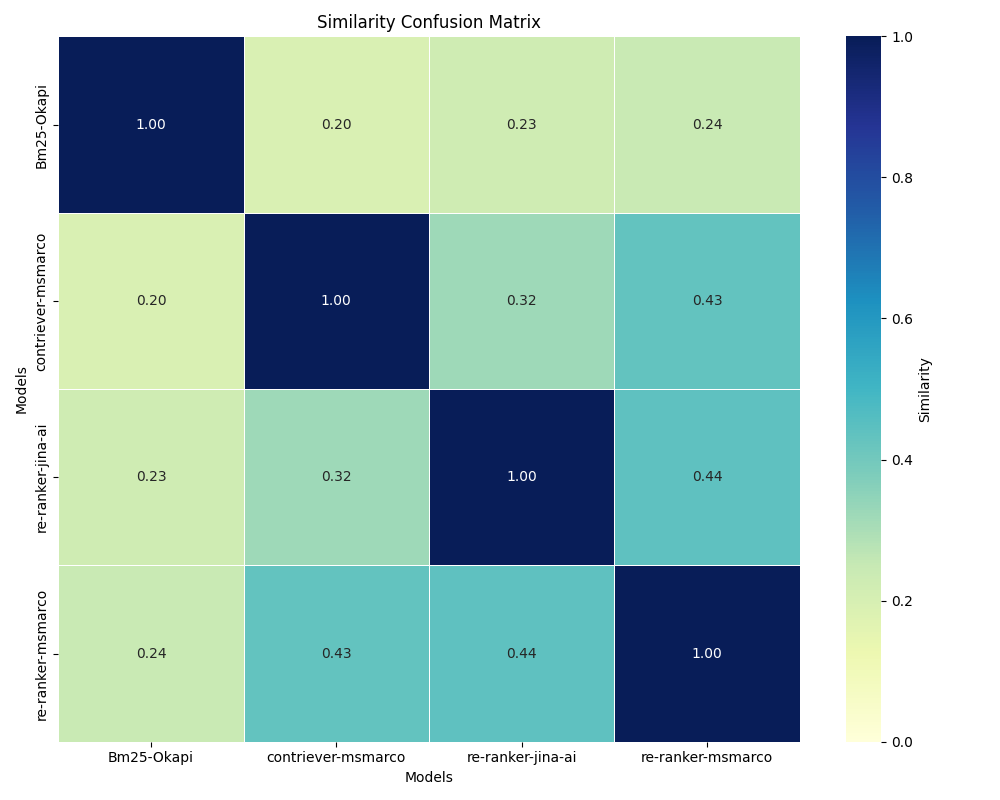
\includegraphics[width=\textwidth]{res/ret_result_sim_1}
        \caption{Document Retrieval Confusion Matrix}
        \label{fig:document_retrieval_confusion_matrix_1}
    \end{minipage}
%    \hspace{0.05\textwidth} % Space between the images
%    \begin{minipage}[b]{0.45\textwidth}
%        \centering
%        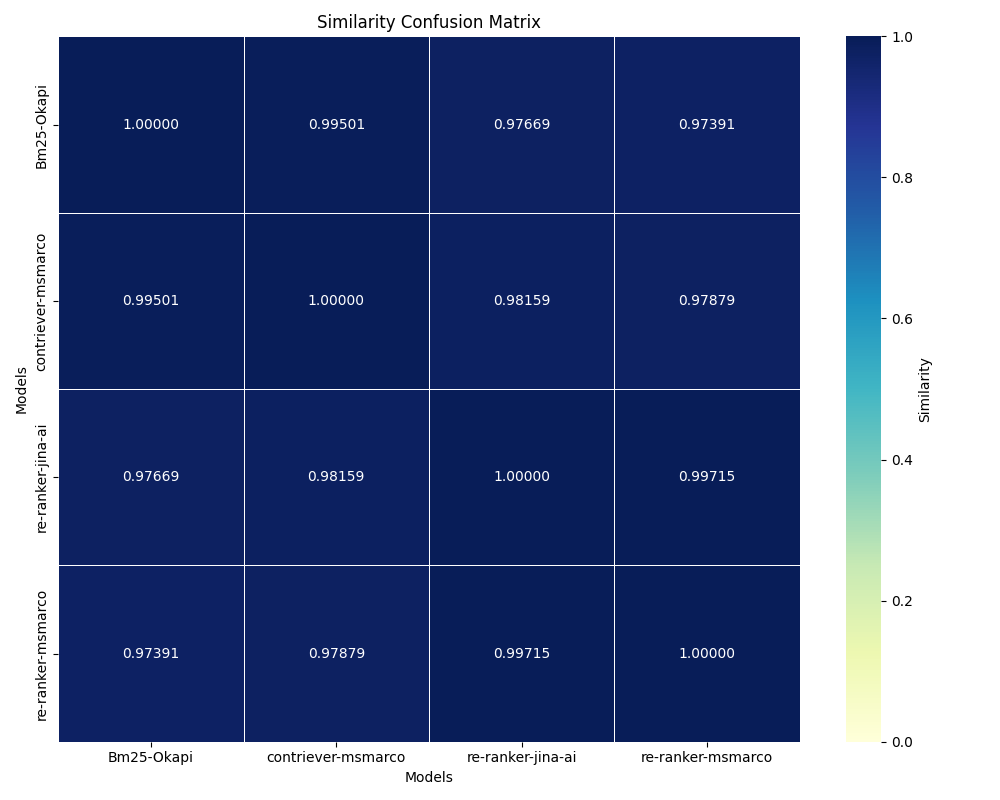
\includegraphics[width=\textwidth]{res/ret_result_sim_2}
%        \caption{Document Retrieval Performance}
%        \label{fig:document_retrieval_confusion_matrix_2}
%    \end{minipage}
\end{figure}

To assess the quality of the retrieved documents from each of the above methods, we are passing them through one of our models and evaluating the outputs.

\begin{table}[h!]
    \centering
    \noindent
    {\scriptsize \fbox{\textit{Retrieval Method}}}\\
    \resizebox{0.7\textwidth}{!}{
        \begin{threeparttable}
        \begin{tabular}{lccc}
            \toprule
            \textbf{Method} & Acc & F1 & Latency\tnote{*} \\
            \midrule
            \textit{Unsupervised}               & & & \\
            Bm25                                & 0.8882          & 0.8940          & \textbf{0.4614s} \\
            contriever-msmarco                  & 0.8932          & 0.8988          & 25.903s \\
            \hline
            \textit{supervised}                 & & & \\
            jina-reranker-v2-base-multilingual  & 0.9004          & 0.9065          & 9.8958s \\
            ms-marco-MiniLM-L-6-v2              & \textbf{0.9014} & \textbf{0.9077} & 0.8172s \\
            \bottomrule
        \end{tabular}
        \begin{tablenotes}
            \item[*] It is measured in seconds on average per query.
        \end{tablenotes}
        \end{threeparttable}}
    \caption{Evaluation Results for Different Retrieval Methods through the Pipeline (just with the Gemma2 model)}
    \label{tab:evaluation_results}
\end{table}

The empirical results indicate that the model \textit{ms-marco-MiniLM-L-6-v2} achieved the highest F1 score, thus demonstrating superior performance among the evaluated models.
However, it is noteworthy that the performance metrics across all models were closely clustered, suggesting that even traditional methodologies applied within our pipeline yield satisfactory outcomes.

It is crucial to emphasize the significance of data quality in this context, as it substantially influences the efficacy of the results.
To validate the factual accuracy of the knowledge graph, we employed a multi-query information fetching through web search engines for each fact.
This approach provides a reasonable degree of verification for the facts contained within the knowledge graph.

For subsequent evaluations and analyzes, we will designate the model \textit{ms-marco-MiniLM-L-6-v2} as our baseline for retrieval tasks.
This decision is predicated on its superior accuracy and F1 score relative to the other models under consideration with acceptable latency.


\section{Embedding Models}\label{sec:embedding-models}
Text embeddings are dense vector representations that capture the semantic meaning and relationships between words, sentences, or documents in a low-dimensional space.
By mapping text to a continuous vector space, embeddings enable efficient similarity computations and have become a fundamental building block for many NLP applications, such as information retrieval, text classification, clustering, and semantic search.
This section provides an in-depth analysis and comparison of five state-of-the-art text embedding models:

\begin{itemize}
    \item Alibaba-NLP/gte-large-en-v1.5
    \item jinaai/jina-embeddings-v3
    \item dunzhang/stella\_en\_1.5B\_v5
    \item Nextcloud-AI/multilingual-e5-large-instruct
    \item BAAI/bge-small-en-v1.5
\end{itemize}

These models leverage recent advancements in transformer architectures, contrastive learning, and instruction fine-tuning to produce high-quality, general-purpose embeddings that excel across a wide range of downstream tasks.
We examine their model architectures, training methodologies, supported features, and empirical performance on standard benchmarks.
Through this comparative study, we aim to provide insights and guidance for practitioners to select the most suitable embedding model based on their specific use case and computational constraints.

\subsection{Gte-large-en-v1.5}\label{subsec:alibaba-nlp}
The Alibaba-NLP model \textit{gte-large-en-v1.5} is text embedding model designed for general text representation and retrieval tasks.
It is built upon a Transformer++ encoder architecture, combining the strengths of BERT~\cite{devlin2019bertpretrainingdeepbidirectional} with advanced techniques such as \ac{RoPE}~\cite{su2023roformerenhancedtransformerrotary} and Gated Linear Units (GLU).
This combination allows for highly efficient text encoding over long sequences, with a maximum context length of 8192 tokens, significantly surpassing previous models restricted to shorter context lengths (up to 512 tokens)~\cite{zhang2024mgtegeneralizedlongcontexttext}.

One of the major improvements in the gte-v1.5 series is its ability to process long-context text inputs, making it ideal for complex text retrieval and re-ranking tasks, especially in multilingual settings~\cite{li2023generaltextembeddingsmultistage}.
This series of models has demonstrated superior performance in multiple benchmarks, including the \ac{MTEB}~\cite{muennighoff-etal-2023-mteb} and the LoCo long-context retrieval benchmark~\cite{saadfalcon2024benchmarkingbuildinglongcontextretrieval}.
In particular, the model ranked second on the MTEB leaderboard and first in the Chinese version of MTEB (C-MTEB).

The model achieves these results by employing a hybrid architecture, including both a text representation model (TRM) and a cross-encoder reranker.
The TRM generates dense text embeddings for retrieval tasks, while the reranker refines results through more precise scoring of candidate texts.
This architecture is optimized for efficiency, allowing faster inference while maintaining high accuracy during both pretraining and fine-tuning stages.

The \textit{gte-large-en-v1.5} also includes instruction-tuned variants, such as \textit{gte-Qwen1.5-7B-instruct}, which is particularly effective for multilingual text embeddings, leveraging a wide range of unsupervised and supervised contrastive learning techniques.
These instruction-tuned models have outperformed various other large embedding models, making them highly suitable for industrial applications that require efficient, accurate text representation across diverse languages.

In summary, the \textit{gte-large-en-v1.5} model stands out in its category due to its ability to handle large context lengths, its efficient encoding techniques, and its strong performance across multilingual and long-context benchmarks.
This makes it an invaluable tool for a variety of text retrieval, classification, and representation tasks in both academic research and real-world applications.

\subsection{Jina-embeddings-v3}\label{subsec:jinaai}
The \textit{Jina-embeddings-v3} model is a cutting-edge multilingual text embedding solution, developed by Jina AI, aimed at addressing a wide range of \ac{NLP} tasks.
Based on the \textit{Jina-XLM-RoBERTa} architecture, this model supports long-context inputs, handling sequences of up to 8192 tokens thanks to its integration of \ac{RoPE}~\cite{su2023roformerenhancedtransformerrotary,sturua2024jinaembeddingsv3multilingualembeddingstask}.

This ability to process extended sequences makes the model well-suited for tasks such as text retrieval, clustering, classification, and text matching across multiple languages.
One of the key innovations of \textit{Jina-embeddings-v3} is the introduction of task-specific \ac{LoRA}~\cite{hu2022lora} adapters.
These adapters are used to tailor the model's embeddings to specific tasks, such as query-document retrieval, clustering, re-ranking, and classification.
This task-specific optimization is achieved without significantly increasing the model's parameter size.

The model excels in multilingual environments, supporting over 30 languages, and is optimized for performance in long-context retrieval tasks.
Compared to LLMs like \textit{e5-mistral-7b-instruct}, \textit{jina-embeddings-v3} offers a more efficient solution with fewer parameters (570 million vs. 7.1 billion), while still achieving competitive or superior performance on several benchmarks.
For example, it surpasses proprietary models like OpenAI~\footnote{\url{https://openai.com/}} and Cohere~\footnote{\url{https://cohere.com/}} on English tasks and achieves high scores on multilingual benchmarks.

\textit{Jina-embeddings-v3} also features flexible \ac{MRL}~\cite{kusupati2024matryoshkarepresentationlearning}, allowing users to reduce the embedding size from 1024 to as low as 32 dimensions, making it adaptable to different resource constraints without significant loss of performance.

\subsection{Stella\_en\_1.5B\_v5}\label{subsec:dunzhang}
The Dunzhang \textit{Stella\_en\_1.5B\_v5}\footnote{\url{https://huggingface.co/dunzhang/stella_en_1.5B_v5}} is a powerful multilingual text embedding model, built upon the foundations of \textit{Alibaba-NLP/gte-large-en-v1.5}~\ref{subsec:alibaba-nlp} and \textit{gte-Qwen2-1.5B-instruct}.
This model supports two main prompts for diverse tasks: "s2p" (sentence-to-passage) for information retrieval, and "s2s" (sentence-to-sentence) for semantic textual similarity. 
These prompts simplify its application in NLP tasks, such as retrieving relevant passages or finding semantically similar text based on a given query.

One of the standout features of \textit{Stella\_en\_1.5B\_v5} is its implementation of \ac{MRL}~\cite{kusupati2024matryoshkarepresentationlearning}, allowing the model to output embeddings in multiple dimensions ranging from 512 to 8192, depending on user needs. 
Typically, a 1024-dimensional output offers an optimal balance between performance and efficiency. 
In benchmark tests, the model achieves highly competitive results, with only a minor performance difference between 1024-dimensional and 8192-dimensional embeddings.
The model can be employed using both SentenceTransformers and transformers libraries, supporting flexible input formats. 
It is trained on shorter sequences (up to 512 tokens), making it most effective for short-to-medium-length text tasks. 

\subsection{Multilingual-e5-large-instruct}\label{subsec:nextcloud-ai}
The Multilingual E5-Large-Instruct model is an advanced multilingual text embedding model introduced as part of the E5 model family, which aims to improve the quality and utility of multilingual text embeddings~\cite{wang2024multilinguale5textembeddings}.
It is specifically designed to support a wide range of languages and to deliver robust performance across various tasks such as text retrieval, semantic similarity, and multilingual retrieval.

The E5-Large-Instruct model contains 24 layers and features an embedding size of 1024.
It builds on the \textit{XLM-RoBERTa-large}~\cite{DBLP:journals/corr/abs-1911-02116} architecture, which supports 100 languages, albeit with varying performance depending on the resource richness of the language in question.
The model was initialized from XLM-RoBERTa-large and underwent two key stages of training:
\begin{itemize}
    \item \textbf{Contrastive Pre-training:} The model was pre-trained on approximately 1 billion weakly supervised multilingual text pairs using a contrastive loss function with a temperature of 0.01. This stage aimed to align similar texts in a shared embedding space.
    \item \textbf{Fine-tuning:} Following pre-training, the model was fine-tuned using high-quality labeled datasets from the E5-mistral paper. This second stage involved a more supervised approach, optimizing performance across specific tasks. During this phase, instruction-tuning was incorporated, where the model learned to generate better embeddings by using natural language task instructions.
\end{itemize}
The E5-Large-Instruct model was evaluated on BEIR and MTEB benchmarks, and its performance is on par with state-of-the-art English-only models.
Evaluation on the MIRACL~\cite{zhang-etal-2023-miracl} multilingual retrieval benchmark across 16 languages and on Bitext mining tasks across over 100 languages demonstrated its capability to handle diverse languages effectively.
Despite the excellent performance on high-resource languages, the model shows degradation in performance for low-resource languages, a common limitation of multilingual models.
The use of contrastive learning and instruction tuning enables the model to generate highly effective embeddings for information retrieval tasks.
However, the absolute cosine similarity values generated by the model are less critical than the relative order of these values, which is more relevant for retrieval and similarity ranking tasks.

%TODO: NEED TO BE UPDATED
\subsection{bge-small-en-v1.5}\label{subsec:baai}
The \textit{\textit{bge-small-en-v1.5}} model is part of the BGE (BAAI General Embeddings) series developed by the Beijing Academy of Artificial Intelligence~\cite{bge_embedding}.
It is a compact English-specific model with just 25M parameters, making it highly efficient for deployment in resource-constrained environments.
The model architecture is based on RoBERTa~\cite{liu2019robertarobustlyoptimizedbert} with optimizations like dynamic token pruning and embedding factorization to reduce computational costs.

\textit{\textit{bge-small-en-v1.5}} follows a two-stage training pipeline similar to other BGE models:
\begin{itemize}
    \item \textbf{Pre-training:} Weakly-supervised contrastive pre-training on large-scale web data
    \item \textbf{Fine-tuning:} Supervised fine-tuning on a curated set of high-quality English NLP datasets
\end{itemize}

The pre-training stage leverages diverse data sources like Wikipedia, Reddit, and CommonCrawl to learn general-purpose text representations. The fine-tuning stage incorporates datasets spanning retrieval, classification, paraphrase detection, and semantic textual similarity tasks to instill task-specific knowledge.

Despite its small size, \textit{\textit{bge-small-en-v1.5}} punches above its weight on several English benchmarks.
On the SentEval suite~\cite{conneau2018senteval}, it outperforms the base-sized BERT and RoBERTa models on most tasks while being 4x more compact.
On retrieval challenges like BEIR, it achieves competitive results, often surpassing larger models like MPNet and the original DPR.
The model's strong performance can be attributed to the efficient architecture design and the use of high-quality fine-tuning data.
It presents an attractive option for applications requiring low-latency inference or deployment on edge devices.

\subsection{Comparative Analysis}\label{subsec:comparative-analysis}
We examine their model size and efficiency, language coverage, supported features, and overall performance to provide insights for selecting the most suitable model based on specific requirements.

\subsubsection{Model Size and Efficiency}
Table~\ref{tab:comparison-embeddings} compares the model size, memory usage, embedding dimensions, and maximum token length of the five models. 
The \textit{stella\_en\_1.5B\_v5} model has the largest size with 1,543 million parameters, while \textit{bge-small-en-v1.5} is the smallest with only 33 million parameters.
Larger models generally require more memory and computational resources, which may be a consideration for resource-constrained environments.
In terms of memory usage, \textit{stella\_en\_1.5B\_v5} requires 5.75 GB in fp32 precision, while \textit{bge-small-en-v1.5} only needs 0.12 GB.
This substantial difference in memory footprint can be a decisive factor when deploying models on edge devices or serving them in real-time applications with limited resources.
The embedding dimensions also vary among the models, ranging from 384 for \textit{bge-small-en-v1.5} to 8192 for \textit{stella\_en\_1.5B\_v5}.
Higher-dimensional embeddings can capture more fine-grained semantic information but may increase storage requirements and similarity computation costs.
Practitioners should consider the trade-off between embedding quality and efficiency based on their specific use case.

\begin{table}[ht!]
    \centering
    \noindent
    \resizebox{\textwidth}{!}{
        \begin{tabular}{lcccc}
            \toprule
            \textbf{Model} & \shortstack{\textbf{Model Size} \\ (Million Parameters)}           & \shortstack{\textbf{Memory Usage} \\ (GB, fp32)}             & \shortstack{\textbf{Embedding}  \\ \textbf{Dimensions}}              & \shortstack{\textbf{Max}  \\ \textbf{Tokens}} \\
            \midrule
            stella\_en\_1.5B\_v5              & 1543   & 5.75 & 8192  & 131072  \\
            jina-embeddings-v3              & 572   & 2.13 & 1024  & 8194  \\
            gte-large-en-v1.5              & 434   & 1.62 & 1024  & 8192  \\
            multilingual-e5-large-instruct              & 560   & 2.09 & 1024  & 514  \\
            bge-small-en-v1.5              & 33   & 0.12 & 384  & 51262  \\
            \bottomrule
        \end{tabular}}
    \caption{Comparison of Embedding Models}
    \label{tab:comparison-embeddings}
\end{table}

\subsubsection{Language Coverage}
Language coverage is a crucial aspect when selecting an embedding model for multilingual applications. The \textit{Multilingual-e5-large-instruct} model stands out in this regard, as it supports a wide range of languages. This model leverages instruction fine-tuning on multilingual data, enabling it to generate high-quality embeddings for various languages.
The \textit{Jina-embeddings-v3} model also offers multilingual support, although the exact language coverage is not specified in the provided context. On the other hand, the \textit{Bge-small-en-v1.5}, \textit{Stella\_en\_1.5B\_v5}, and \textit{Gte-large-en-v1.5} models primarily focus on English embeddings, making them more suitable for monolingual English applications.

\subsubsection{Supported Features}
The embedding models offer various features that cater to different use cases. The \textit{Stella\_en\_1.5B\_v5} model supports two main prompts for diverse tasks: "s2p" (sentence-to-passage) for information retrieval and "s2s" (sentence-to-sentence) for semantic textual similarity. This flexibility allows users to adapt the model for specific NLP tasks with minimal effort.
The \textit{Jina-embeddings-v3} model incorporates task-specific LoRA adapters, enabling it to generate high-quality embeddings for query-document retrieval, clustering, classification, and text matching. This feature eliminates the need for manual prompt engineering and provides a more streamlined approach for task-specific embeddings.
Additionally, the \textit{Stella\_en\_1.5B\_v5} and \textit{Jina-embeddings-v3} models implement MRL, allowing users to generate embeddings with different dimensions based on their needs. This adaptability is particularly useful when balancing between embedding quality and storage or computational efficiency.

\subsubsection{Conclusion}
The choice of text embedding model depends on various factors, including the specific application, language coverage requirements, available computational resources, and desired features. For monolingual English applications, the \textit{Gte-large-en-v1.5} and \textit{Stella\_en\_1.5B\_v5} models offer high-quality embeddings with support for longer input sequences.
The \textit{Stella\_en\_1.5B\_v5} model, in particular, provides prompt-based adaptability for information retrieval and semantic similarity tasks.
For multilingual applications, the \textit{Multilingual-e5-large-instruct} and \textit{Jina-embeddings-v3} models are strong contenders.
The \textit{Multilingual-e5-large-instruct} model supports a wide range of languages, while \textit{Jina-embeddings-v3} offers task-specific LoRA adapters for enhanced performance across various NLP tasks.
When computational resources are limited, the \textit{Bge-small-en-v1.5} model presents a lightweight option with competitive performance.
Its small size and low memory footprint make it suitable for deployment on edge devices or real-time applications.
Ultimately, practitioners should carefully evaluate their specific requirements and constraints before selecting an embedding model.
The comparative analysis provided in this section aims to assist in this decision-making process by highlighting the key differences and strengths of each model.

Now we will test these models through the pipeline and evaluate their performance.

\begin{table}[h!]
    \centering
    \noindent
    {\scriptsize ms-marco-MiniLM-L-6-v2,\fbox{\textit{Embedding Model}}}\\
    \resizebox{0.7\textwidth}{!}{
        \begin{threeparttable}
        \begin{tabular}{lccc}
            \toprule
            \textbf{Model} & Acc & F1 & Latency \\
            \midrule
            stella\_en\_1.5B\_v5                  & 0.8961          & 0.9028          & 17.692s \\
            jina-embeddings-v3\tnote{*}           & 0.8852          & 0.9097          & 4.8745s \\
            gte-large-en-v1.5\tnote{*}            & 0.8971          & \textbf{0.9174} & 5.8571s \\
            multilingual-e5-large-instruct        & 0.8954          & 0.9018          & 5.0038s \\
            bge-small-en-v1.5                     & \textbf{0.9014} & 0.9077          & \textbf{1.6958s} \\
            \bottomrule
        \end{tabular}
        \begin{tablenotes}
            \item[*] The models were not able to complete the evaluation due to memory constraints, Jina evaluated on the 2238/2800 and Gte-large evaluated on the 2322/2800.
        \end{tablenotes}
    \end{threeparttable}}
    \caption{Evaluation Results for Different Embedding Models through the Pipeline (just with the Gemma2 model)}
    \label{tab:evaluation_results_embedding}
\end{table}

Based on the Table~\ref{tab:evaluation_results_embedding}, we use the \textit{bge-small-en-v1.5} model for the subsequent evaluations and analyses due to its superior performance across Acc metric, the F1 score of \textit{gte-large-en-v1.5} is slightly higher, but the model is not able to complete the evaluation due to memory limitations in the same pipeline.

\section{Chunking Strategies}\label{sec:chunking-strategies}
A critical component of \ac{RAG} systems is the chunking strategy employed to divide documents into smaller, manageable pieces for efficient retrieval and processing.
This chapter examines three distinct chunking methods for \ac{RAG} systems, each with its unique characteristics and potential advantages.

\subsection{Parsing Documents into Text Chunks}\label{subsec:parsing-documents-into-text-chunks}
The first method we will explore involves parsing documents into text chunks, also referred to as nodes, of fixed sizes.
This approach is straightforward and widely used in many RAG implementations.
We will investigate three different chunk sizes: 256, 512, and 1024 tokens.
\subsubsection{Methodology}
In this method, documents are sequentially divided into chunks of the specified size.
If the final chunk is smaller than the designated size, it is typically padded or left as is, depending on the implementation.
\subsubsection{Chunk Sizes}
\begin{itemize}
    \item \textbf{256-token chunks:} This size offers fine granularity, potentially allowing for more precise retrieval of relevant information. However, it may result in a loss of context for more complex topics that require broader context.
    \item \textbf{512-token chunks:} This medium-sized chunk strikes a balance between granularity and context preservation. It is often considered a good default choice for many applications.
    \item \textbf{1024-token chunks:} Larger chunks preserve more context but may retrieve more irrelevant information and increase computational overhead during retrieval and processing.
\end{itemize}
\subsubsection{Advantages and Limitations}
Advantages:
\begin{enumerate}
    \item Simple to implement and understand
    \item Consistent chunk sizes facilitate uniform processing
\end{enumerate}
Limitations:
\begin{enumerate}
    \item Fixed chunk sizes may not align with natural breaks in the text
    \item Larger chunks can introduce irrelevant information and increase computational costs
\end{enumerate}
\subsection{Smaller Child Chunks Referring to Bigger Parent Chunks (Small2Big)}\label{subsec:smaller-child-chunks-referring-to-bigger-parent-chunks}
The second method, which we will refer to as \textit{Small2Big}, involves creating a hierarchical structure of chunks, where smaller child chunks refer to larger parent chunks.
This approach aims to combine the benefits of fine-grained retrieval with the context preservation of larger chunks.
\subsubsection{Methodology}
In this method, we parsed documents into three levels of chunks with appending the original text chunk of size 1024:
\begin{itemize}
    \item Smallest children: 128-token chunks
    \item Intermediate parents: 256-token chunks
    \item Largest parents: 512-token chunks
\end{itemize}
Each smaller chunk maintains a reference to its parent chunks, allowing the system to retrieve additional context when needed.

\begin{lstlisting}[language=Python, caption=Small2Big Chunking Method, label=lst:small2big_chunking]
# ...previous code
sub_chunk_sizes = [128, 256, 512]
sub_node_parsers = [SimpleNodeParser.from_defaults(chunk_size=c) for c in sub_chunk_sizes]

all_nodes = []
for base_node in base_nodes:
    for n in sub_node_parsers:
        sub_nodes = n.get_nodes_from_documents([base_node])
        sub_inodes = [
            IndexNode.from_text_node(sn, base_node.node_id) for sn in sub_nodes
        ]
        all_nodes.extend(sub_inodes)

    original_node = IndexNode.from_text_node(base_node, base_node.node_id) # also add original node to node
    all_nodes.append(original_node)
all_nodes_dict = {n.node_id: n for n in all_nodes}
# ... continue processing
\end{lstlisting}

\subsubsection{Advantages and Limitations}
Advantages:
\begin{enumerate}
    \item Allows for fine-grained retrieval with the option to expand context
    \item Adapts to different levels of specificity required by queries
\end{enumerate}
Limitations:
\begin{enumerate}
    \item More complex to implement and manage
    \item Increased storage requirements due to redundancy in the hierarchy
\end{enumerate}
\subsection{Sentence Window Retrieval}\label{subsec:sentence-window-retrieval}
The third method, Sentence Window Retrieval, focuses on maintaining semantic coherence by chunking based on sentences and incorporating surrounding context through windows.
\subsubsection{Methodology}
In this approach, documents are first split into individual sentences.
For each sentence, a \textit{window} of surrounding sentences is included to provide context.
We will examine two window sizes: 3 and 6.
For each sentence, the chunk includes the sentence itself, one preceding sentence, and one following sentence.

\subsubsection{Advantages and Limitations}
Advantages:
\begin{enumerate}
    \item Preserves semantic units (sentences) and their immediate context
    \item Adapts to the natural structure of the text
\end{enumerate}
Limitations:
\begin{enumerate}
    \item Variable chunk sizes may complicate processing and indexing
    \item Optimal window size may vary depending on the document type and content
\end{enumerate}
\subsection{Evaluation}\label{subsec:evaluation}
Each of the three chunking methods presented in this chapter offers distinct advantages and limitations for RAG systems. 
The choice of method depends on factors such as the nature of the documents, the specific requirements of the application, and the computational resources available.
The fixed-size chunking method provides simplicity and consistency but may sacrifice semantic coherence. 
The Small2Big hierarchical approach offers flexibility in retrieval granularity but introduces complexity in implementation and storage. 
Sentence Window Retrieval preserves semantic units and adapts to text structure but may result in variable chunk sizes.

\begin{table}[h!]
    \centering
    \noindent
    {\scriptsize ms-marco-MiniLM-L-6-v2, BAAI/bge-small-en-v1.5,\fbox{\textit{Chunking Strategy}}}\\
    \resizebox{0.75\textwidth}{!}{
        \begin{tabular}{llccc}
            \toprule
            \textbf{Method} & \textbf{Parameters} & Acc & F1 & Latency \\
            \midrule
            \multirow{3}{*}{Original}           & Chuck Size: 256       & 0.8914          & 0.8914          & 0.04473s \\
                                                & Chuck Size: 512       & 0.8932          & 0.8993          & 0.02670s \\
                                                & Chuck Size: 1024      & 0.8946          & 0.8993          & \textbf{0.02378s} \\ \hline
            small2big                           & Chuck Size: 1024      & 0.8889          & 0.8953          & 0.19188s \\ \hline

            \multirow{2}{*}{Sliding Window}     & Window Size: 3        & \textbf{0.9014} & \textbf{0.9080} & 0.03076s \\
                                                & Window Size: 6        & \textbf{0.9014} & 0.9077          & 0.03534s \\
            \bottomrule
        \end{tabular}}
    \caption{Evaluation Results for Different Chunking Strategies through the Pipeline (just with the Gemma2 model)}
    \label{tab:table_chunking}
\end{table}
Examples of the three chunking methods are available in the Appendix~\ref{ch:chunking} for further reference.

The high baseline accuracy and F1 scores across chunking strategies indicate that the model’s performance is largely unaffected by these variations, suggesting that factors other than chunk size, may have a more significant impact on the retrieval process.
The Sliding Window method with a window size of 3 achieves the highest accuracy and F1 score, so we will use this method for subsequent evaluations and analyses due to its F1, accuracy scores and having surrounding context.

\section{Similarity Cut-off}\label{sec:similar-cut-off}
In this section we will discuss how similarity cut-off can be used to filter out irrelevant nodes and improve the efficiency of the retrieval process.
We use Node postprocessors to apply a similarity cut-off to the retrieved nodes, discarding those with a similarity score below a certain threshold.
Node postprocessors are a set of modules that take a set of nodes, and apply some kind of transformation or filtering before returning them.
For our experiments, we set the similarity cut-off threshold to 0.3, meaning that nodes with a similarity score below 0.3 are discarded, we use the naive score and the re-ranker score to compare the results.

\begin{algorithm}
    \begin{algorithmic}[1]
        \Procedure{PostprocessNodes}{nodes, knowledge\_graph, similarity\_cutoff}
            \State $new\_nodes \gets []$
            \State $node\_texts \gets [node.text \text{ for } node \text{ in } nodes]$
            \State $re\_rank\_nodes \gets \textsc{ReRank}(knowledge\_graph, node\_texts)$

            \For{each $node$ in $nodes$}
                \State $node.score \gets \text{get\_node\_score}(node.text, re\_rank\_nodes)$

                \If{$node.score > similarity\_cutoff$}
                    \State $new\_nodes.\textsc{Append}(node)$
                \EndIf
            \EndFor

            \State \Return $new\_nodes$
        \EndProcedure
    \end{algorithmic}
    \caption{Similarity Cutoff Postprocessor}\label{alg:algorithm}
\end{algorithm}

\begin{table}[h!]
    \centering
    \noindent
    {\scriptsize ms-marco-MiniLM-L-6-v2, BAAI/bge-small-en-v1.5, Sliding Window (ws 3), \fbox{\textit{Similarity Cut-off}}}\\
    \resizebox{0.7\textwidth}{!}{
        \begin{threeparttable}
        \begin{tabular}{lccc}
            \toprule
            \textbf{Method} & Acc & F1 & Latency\tnote{*} \\
            \midrule
            w/o similarity cut-off                                  & 0.8971          & 0.9036                  &  N/A \\
            similarity cut-off (original score)                     & \textbf{0.9018} & \textbf{0.9080}         & -0.22237s \\
            similarity cut-off (re-ranked score)                    & 0.9014          & \textbf{0.9080}         & -0.350783 \\
            \bottomrule
        \end{tabular}
        \begin{tablenotes}
            \item[*] The latency is compared to the baseline without the similarity cut-off on average per query.
        \end{tablenotes}
    \end{threeparttable}}
    \caption{Evaluation Results for Different Similarity Cut through the Pipeline (just with the Gemma2 model)}
    \label{tab:table_similarity_cut}
\end{table}

Based on the results in Table~\ref{tab:table_similarity_cut}, we apply a similarity cut-off on the original score to provide the model with higher-quality data for further evaluations.
This approach yields the highest accuracy and F1 score, though it is slightly slower than the re-ranker mode because it removes more irrelevant nodes.
A drawback of re-ranking is that it may eliminate all relevant nodes with low similarity scores, requiring a re-run without the similarity cut-off, which increases processing time (not shown in the table).
Additionally, in separate evaluations (not reported in Table~\ref{tab:table_similarity_cut}), we tested a normalized similarity cut-off using re-ranked scores scaled between the original minimum and maximum values.
However, this normalized approach did not perform as well as the original scores.
\section{Top K}\label{sec:top-k}
Top\_k mentions how many top embeddings to take into context.
Considering a large top\_k might go beyond the max\_tokens of the model, we will evaluate the performance of the pipeline with the top\_k set to 3 and 6, and compare the results to determine the optimal value for this parameter.
\begin{table}[h!]
    \centering
    \noindent
    {\scriptsize ms-marco-MiniLM-L-6-v2, BAAI/bge-small-en-v1.5, Sliding Window (ws 3), Similarity Cut-off (Original),\fbox{\textit{Top\_k}}}
    \resizebox{0.4\textwidth}{!}{
        \begin{threeparttable}
        \begin{tabular}{lccc}
            \toprule
            \textbf{Method} & Acc & F1 & Latency\tnote{*} \\
            \midrule
            Top\_k 3                     & 0.9018               & 0.9080                    & \textbf{5.21177s} \\
            Top\_k 6                     & \textbf{0.9032}      & \textbf{0.9101}           & 7.02713s \\
            \bottomrule
        \end{tabular}
        \begin{tablenotes}
            \item[*] The latency represents the average time per query for a complete run.
        \end{tablenotes}
        \end{threeparttable}}
    \caption{Evaluation Results for Different Top\_k through the Pipeline (just with the Gemma2 model)}
    \label{tab:table_top_k}
\end{table}

As we decided to set the similarity cut-off with 0.3 threshold, it's good to use the top\_k 6 to have more high-quality embeddings in the context, and based on results it outperforms the top\_k 3, so we will use top\_k 6 for subsequent evaluations.
The difference in latency is significant, presenting a trade-off between accuracy and processing time.
Since the quality of data for additional facts is uncertain, we aim to include more data in the context.

\section{Evaluation}\label{sec:evaluation-and-discussion}
In this ablation study, we evaluate the performance of the merging method, which leverages a novel ensemble approach by combining multiple models (Gemma2, Qwen2.5, Llama3.1, and Mistral) to show the robustness and accuracy of the pipeline.
As presented in Tables~\ref{tab:evaluation_results-full-category} and~\ref{tab:evaluation_results-full-wo-category}, along with Figures~\ref{fig:correct-radar-chart}, ~\ref{fig:wrong-radar-chart}, and ~\ref{fig:all-radar-chart}, the proposed ensemble method consistently outperforms individual models across both positive and negative labels, achieving a more balanced and comprehensive performance.

Note that the ensemble method is based on the tie-breaking strategy discussed in Section~\ref{subsec:conflict-resolution-strategies}, with \textit{At\_Most} as the merging method.
Based on provided configurations, the model selected for \textit{At\_Most} is the \textit{Gemma2:21B} model.

\begin{table}
    \noindent
    {\scriptsize ms-marco-MiniLM-L-6-v2, BAAI/bge-small-en-v1.5, Sliding Window (ws 3), Similarity Cut-off (Original), Top\_k 6}
    \resizebox{\textwidth}{!}{
        \begin{tabular}{lcccccccccc||c}
            \toprule
            \textbf{Model}                     & \begin{sideways}award\end{sideways}                     & \begin{sideways}birth\end{sideways}                     & \begin{sideways}death\end{sideways}                     & \begin{sideways}foundationPlace\end{sideways}                     & \begin{sideways}leader\end{sideways}                    & \begin{sideways}nbateam\end{sideways}                     & \begin{sideways}publicationDate\end{sideways}                     & \begin{sideways}spouse\end{sideways}                    & \begin{sideways}starring\end{sideways} & \begin{sideways}subsidiary\end{sideways} & \begin{sideways}Total\end{sideways} \\
            \midrule
            \textit{Positive Labels}           &                                                         &                                                         &                                                         &                                                                   &                                                         &                                                           &                                                                   &                                                         &                                        &                                          &       \\
            Gemma2                             & 1.0000                                                  & 0.9733                                                  & 0.9200                                                  & 0.5667                                                            & 0.9933                                                  & 1.0000                                                    & 0.9733                                                            & 0.8000                                                  & 0.9733                                 & 0.9467                                   & 0.9147 \\
            Qwen2.5                            & 1.0000                                                  & 0.9667                                                  & 0.9600                                                  & 0.7800                                                            & 0.9933                                                  & 1.0000                                                    & 0.9600                                                            & 0.9400                                                  & 0.9800                                 & 0.9067                                   & 0.9487 \\
            Llama3.1                           & 0.9800                                                  & 0.8933                                                  & 0.8267                                                  & 0.5067                                                            & 0.9333                                                  & 0.8467                                                    & 0.9267                                                            & 0.7867                                                  & 0.8667                                 & 0.8400                                   & 0.8407 \\
            Mistral                            & 1.0000                                                  & 0.9867                                                  & 0.9667                                                  & 0.7333                                                            & 0.9933                                                  & 0.9867                                                    & 0.9867                                                            & 0.9867                                                  & 0.9867                                 & 0.9533                                   & 0.9580 \\
            Proposed (At\_Most)                & 1.0000                                                  & 0.9867                                                  & 0.9467                                                  & 0.7067                                                            & 0.9933                                                  & 1.0000                                                    & 0.9667                                                            & 0.9200                                                  & 0.9867                                 & 0.9333                                   & 0.9440 \\
            \hline
            \textit{Negative Labels}           &                                                         &                                                         &                                                         &                                                                   &                                                          &                                                           &                                                                  &                                                         &                                        &                                          &       \\
            Gemma2                             & 0.9923                                                  & 0.9538                                                  & 0.9615                                                  & 0.8154                                                            & 0.9308                                                  & 0.6846                                                    & 0.9308                                                            & 0.9462                                                  & 0.9077                                 & 0.7769                                   & 0.8900 \\
            Qwen2.5                            & 0.8000                                                  & 0.9000                                                  & 0.9000                                                  & 0.6769                                                            & 0.8769                                                  & 0.5462                                                    & 0.7923                                                            & 0.8538                                                  & 0.7462                                 & 0.7615                                   & 0.7854 \\
            LLama3.1                           & 0.7462                                                  & 0.8615                                                  & 0.8462                                                  & 0.7615                                                            & 0.8692                                                  & 0.6385                                                    & 0.8538                                                            & 0.7538                                                  & 0.8231                                 & 0.7077                                   & 0.7862 \\
            Mistral                            & 0.6538                                                  & 0.8692                                                  & 0.8462                                                  & 0.7000                                                            & 0.8077                                                  & 0.6077                                                    & 0.6769                                                            & 0.7846                                                  & 0.6846                                 & 0.6462                                   & 0.7277 \\
            Proposed (At\_Most)                & 0.8846                                                  & 0.9308                                                  & 0.9077                                                  & 0.7692                                                            & 0.8923                                                  & 0.6615                                                    & 0.9000                                                            & 0.8846                                                  & 0.8385                                 & 0.7462                                   & 0.8415 \\
            \bottomrule
        \end{tabular}}
    \caption{Pipeline Evaluation Results - Category-wise}
    \label{tab:evaluation_results-full-category}
\end{table}

\begin{table}
    \noindent
    {\scriptsize ms-marco-MiniLM-L-6-v2, BAAI/bge-small-en-v1.5, Sliding Window (ws 3), Similarity Cut-off (Original), Top\_k 6}
    \resizebox{\textwidth}{!}{
        \begin{tabular}{lccc||cc}
            \toprule
            \textbf{Model}                     & \textbf{Stability}             & \textbf{Avg. Request Duration} & \textbf{Avg. tokens per request}          & \textbf{ACC} & \textbf{F1} \\
            \midrule
            Gemma2                             & 0.8720                         & 5.6826s                            & 1605.29                                       & \textbf{0.9032}    & \textbf{0.9101}   \\
            Qwen2.5                            & 0.8685                         & 6.3094s                            & 1652.66                                       & 0.8729    & 0.8888   \\
            LLama3.1                           & 0.8291                         & 6.5270s                            & 1679.04                                       & 0.8154    & 0.8299   \\
            Mistral                            & 0.8650                         & 4.6692s                            & 1594.76                                       & 0.8511    & 0.8733   \\ \hline
            Proposed (At\_Most)                & \textbf{0.9176}                & 16.815s                            & 1604.196                                      & 0.8964    & 0.9071   \\
            \bottomrule
        \end{tabular}}
    \caption{Pipeline Evaluation Results}
    \label{tab:evaluation_results-full-wo-category}
\end{table}

\begin{figure}[ht!]
    \centering
    \begin{minipage}[b]{0.4\textwidth}
        \centering
        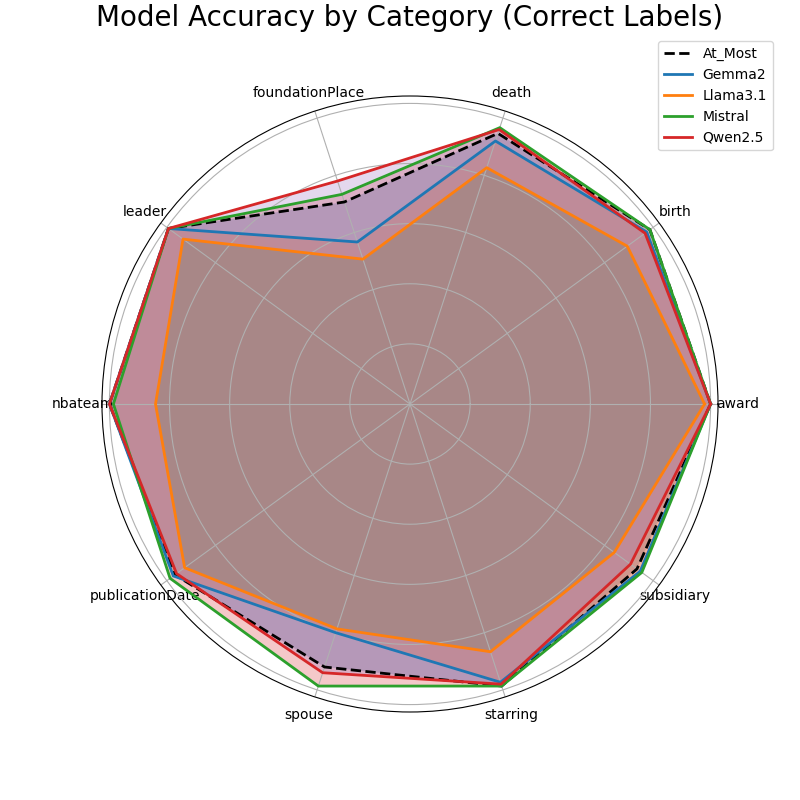
\includegraphics[width=\textwidth]{res/combined_correct_radar_chart}
        \caption{Positive Labels}
        \label{fig:correct-radar-chart}
    \end{minipage}
    \hspace{0.05\textwidth} % Space between the images
    \begin{minipage}[b]{0.4\textwidth}
        \centering
        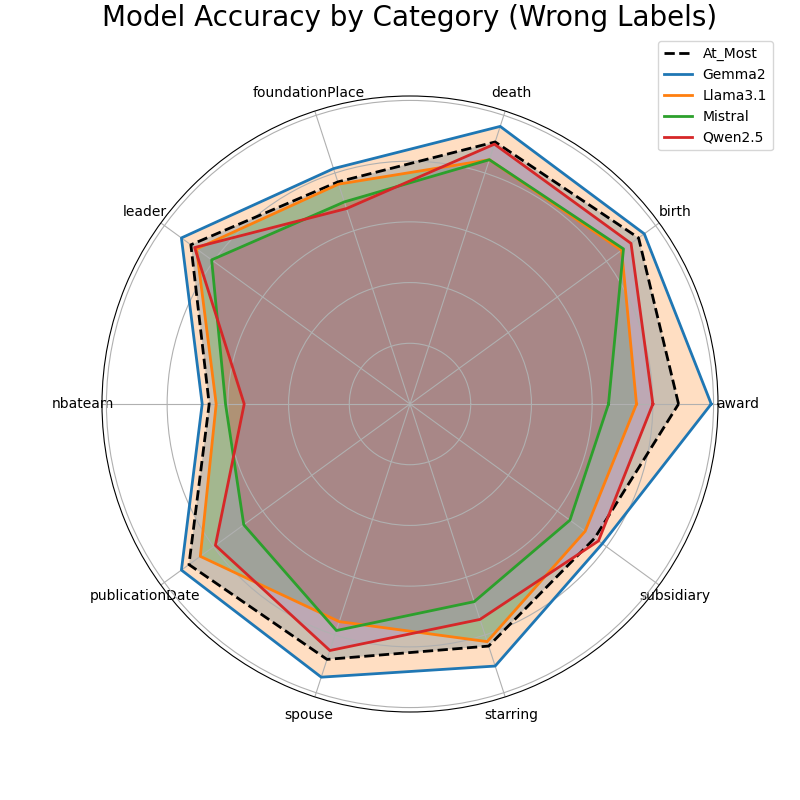
\includegraphics[width=\textwidth]{res/combined_wrong_radar_chart}
        \caption{Negative Labels}
        \label{fig:wrong-radar-chart}
    \end{minipage}
\end{figure}

\begin{figure}[ht!]
    \centering
    \begin{minipage}[b]{0.4\textwidth}
        \centering
        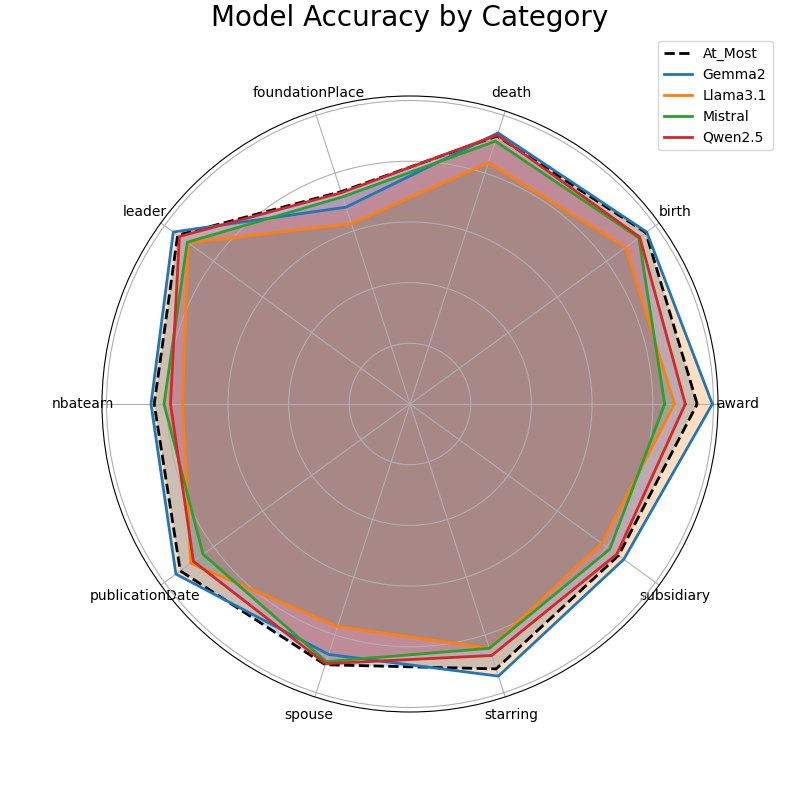
\includegraphics[width=\textwidth]{res/combined_radar_chart}
        \caption{All Labels}
        \label{fig:all-radar-chart}
    \end{minipage}
\end{figure}


\section{Failure Analysis}\label{sec:faiure-analysis}
To gain a deeper understanding of the limitations and challenges faced by our fact-checking system, we conducted a comprehensive failure analysis using the \textit{FactBench} dataset.
By examining the instances where our system, based on the majority vote, failed to correctly verify the facts, we aimed to identify the main error types and provide insights into the reasons behind these failures.
\subsubsection{Error Type Categorization}
After analyzing the failure cases, we categorized the errors into five main types:
\begin{itemize}
    \item \textbf{Insufficient or Irrelevant Context:} In some cases, the provided context information does not directly support or refute the given triple. The LLMs struggle to make accurate judgments when the necessary facts are missing or the available information is tangentially related to the claim.
    \item \textbf{Misinterpretation of Relationships:} The LLMs sometimes misinterpret the relationships between entities mentioned in the context. They may confuse family relations, professional associations, or the nature of events.
    \item \textbf{Over reliance on Keyword Matching:} In some instances, the LLMs rely too heavily on surface-level keyword matching rather than understanding the underlying semantics. The presence of certain words or phrases can lead to incorrect assumptions.
    \item \textbf{Lack of Common Sense Reasoning:} The LLMs can struggle with applying common sense knowledge or reasoning about the plausibility of claims. They may fail to consider the unlikelihood of certain scenarios or relationships.
    \item \textbf{Difficulty with Negation and Contradiction:} The LLMs sometimes struggle with handling negation or identifying contradictions between the triple and the context information. They may overlook explicit denials or fail to recognize inconsistencies.
\end{itemize}

To quantify the distribution of error types, we classified each error instance into one or more of five categories, allowing for overlaps when errors fit multiple categories.
\begin{table}[h!]
    \footnotesize
    \begin{xltabular}{\linewidth}{p{3cm}p{3cm}X}
        \toprule
        \textbf{Error Type} & \textbf{Triple} & \textbf{Description} \\
        \midrule
        Insufficient or Irrelevant Context & Ai Sugiyama birth place Yokohama & Since there's no information in any of the documents about Ai Sugiyama being born in Yokohama, and one document explicitly states her birthplace as Tokyo. So LLms infer that Ai Sugiyama was born in Tokyo, Japan and not Yokohama, Japan. \\
        Mis Interpretation of Relationships & Mitt Romney office Dallas & LLMs mistakenly infer that Romney has an office in Dallas based on his attendance at a fundraiser there. Attending an event doesn't imply having a permanent office. \\
        Over reliance on Keyword Matching & Robbie Williams office Los Angeles & LLMs wrongly assume Robbie Williams has an office in Los Angeles due to text discussing his purchase or sell of a property there, not an office. \\
        Lack of Common Sense Reasoning & Saul Bellow starring Nobel Prize in Literature & LLMs fail to recognize "starring" is inappropriate for receiving a Nobel Prize. Common sense suggests terms like "awarded" or "received." \\
        Difficulty with Negation and Contradiction & John William Strutt team Nobel Prize in Physics & LLMs confirm the presence of a team, despite no evidence suggesting Strutt was part of one. The context mentions Strutt’s Nobel Prize but lacks information about team involvement. \\
        \bottomrule
    \end{xltabular}
    \caption{Examples of Failure Cases and Error Analysis}
    \label{tab:factbench-failure-analysis}
\end{table}

Based on Figures~\ref{fig:wrong_prediction_distribution_0} and~\ref{fig:wong_prediction_distribution_1}, The "foundationPlace" relation shows the highest number of total instances and errors in both charts.
This suggests that the model struggles most with verifying facts about the locations where organizations or institutions were founded.
The large discrepancy between correct and incorrect predictions for this relation indicates a significant challenge in accurately processing location-based information.

Relations such as "birth", "death", and "spouse" show varying levels of difficulty.
While "birth" and "death" have relatively few instances, "spouse" has a moderate number of cases with a notable error rate.
This suggests that verifying personal information, especially relationships, poses challenges for the model, and mostly related to having multiple marriages or relationships during a lifetime.

The "nbateam" and "subsidiary" relations, which involve organizational affiliations, show moderate error rates.
This indicates that the model has some difficulty in correctly identifying professional associations and corporate structures.

\begin{figure}[ht!]
    \centering
    \begin{minipage}[b]{0.4\textwidth}
        \centering
        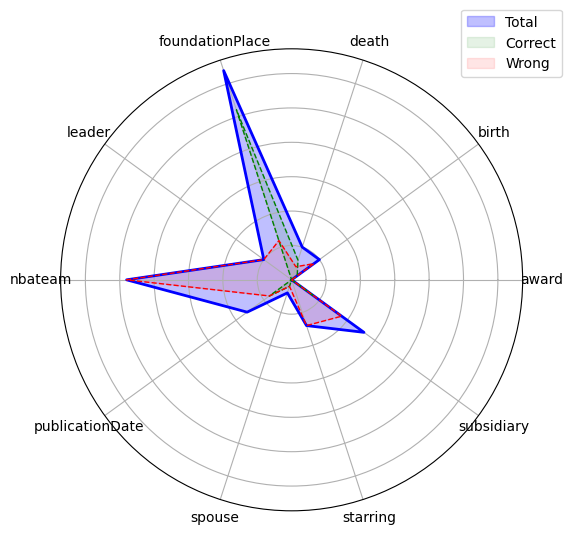
\includegraphics[width=\textwidth]{res/radar-error-0}
        \caption{Distribution of Fully Incorrect Predictions 4/4}
        \label{fig:wrong_prediction_distribution_0}
    \end{minipage}
    \hspace{0.05\textwidth} % Space between the images
    \begin{minipage}[b]{0.4\textwidth}
        \centering
        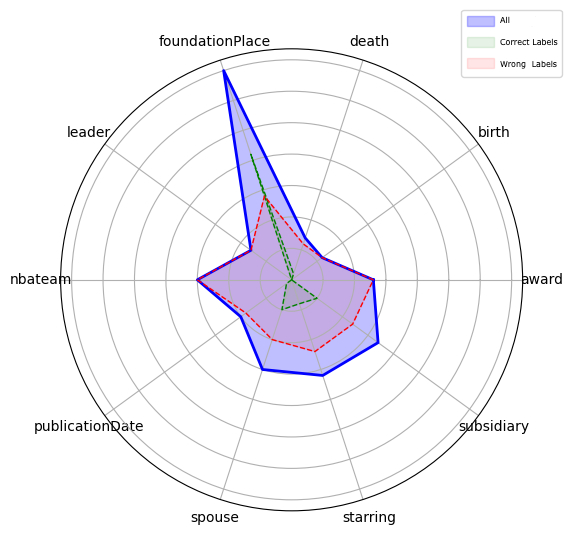
\includegraphics[width=\textwidth]{res/radar-error-1}
        \caption{Distribution of Partially Incorrect Predictions 3/4}
        \label{fig:wong_prediction_distribution_1}
    \end{minipage}
\end{figure}

In general, by comparing Figures~\ref{fig:wrong_prediction_distribution_0} and~\ref{fig:wong_prediction_distribution_1}, we can observe that the overall shape of the error distribution is similar, indicating consistency in the model's performance across different voting thresholds